\documentclass{article}
\usepackage{fontspec}
\setmainfont{Times New Roman}
\usepackage{geometry}
\usepackage{CTEX}
\geometry{papersize={21cm,29.7cm}}
\geometry{left=3.18cm,right=3.18cm,top=2.54cm,bottom=2.54cm}
\usepackage{fancyhdr}
\usepackage{amsmath}
\pagestyle{fancy}
\lhead{学号:202000460020}
\rhead{姓名:苏博南}
\cfoot{\thepage}
\renewcommand{\headrulewidth}{0.4pt}
\renewcommand{\headwidth}{\textwidth}
\usepackage{tikz}
\usetikzlibrary{automata, positioning, arrows}
\usepackage{listings}

\newtheorem{question}{题目}  
\lstset{
	basicstyle=\small\ttfamily,	% 基本样式
		keywordstyle=\color{blue}, % 关键词样式
		commentstyle=\color{gray!50!black!50},   	% 注释样式
		stringstyle=\rmfamily\slshape\color{red}, 	% 字符串样式
	backgroundcolor=\color{gray!0},     % 代码块背景颜色
	frame=leftline,						% 代码框形状
	framerule=12pt,%
		rulecolor=\color{gray!0},      % 代码框颜色
	numbers=left,				% 左侧显示行号往左靠, 还可以为right ,或none,即不加行号
		numberstyle=\footnotesize\itshape,	% 行号的样式
		firstnumber=1,
		stepnumber=1,                  	% 若设置为2,则显示行号为1,3,5
		numbersep=7pt,               	% 行号与代码之间的间距
	aboveskip=.25em, 			% 代码块边框
	showspaces=false,               	% 显示添加特定下划线的空格
	showstringspaces=false,         	% 不显示代码字符串中间的空格标记
	keepspaces=true, 					
	showtabs=false,                 	% 在字符串中显示制表符
	tabsize=2,                     		% 默认缩进2个字符
	captionpos=b,                   	% 将标题位置设置为底部
	flexiblecolumns=true, 			%
	breaklines=true,                	% 设置自动断行
	breakatwhitespace=false,        	% 设置自动中断是否只发生在空格处
	breakautoindent=true,			%
	breakindent=1em, 			%
	title=\lstname,				%
	escapeinside=``,  			% 在``里显示中文
	xleftmargin=1em,  xrightmargin=1em,     % 设定listing左右的空白
	aboveskip=1ex, belowskip=1ex,
	framextopmargin=1pt, framexbottommargin=1pt,
        abovecaptionskip=-2pt,belowcaptionskip=3pt,
	% 设定中文冲突,断行,列模式,数学环境输入,listing数字的样式
	extendedchars=false, columns=flexible, mathescape=true,
	texcl=true,
	fontadjust
}%

\begin{document}

\begin{center}
    \huge{机器学习课程实验四}\\
    \large{\today \quad 苏博南\quad 202000460020}
\end{center}

\section{数据打印}
利用Matlab工具载入并打印数据,得到如下图1所示结果

\begin{figure}[h]
    \centering
    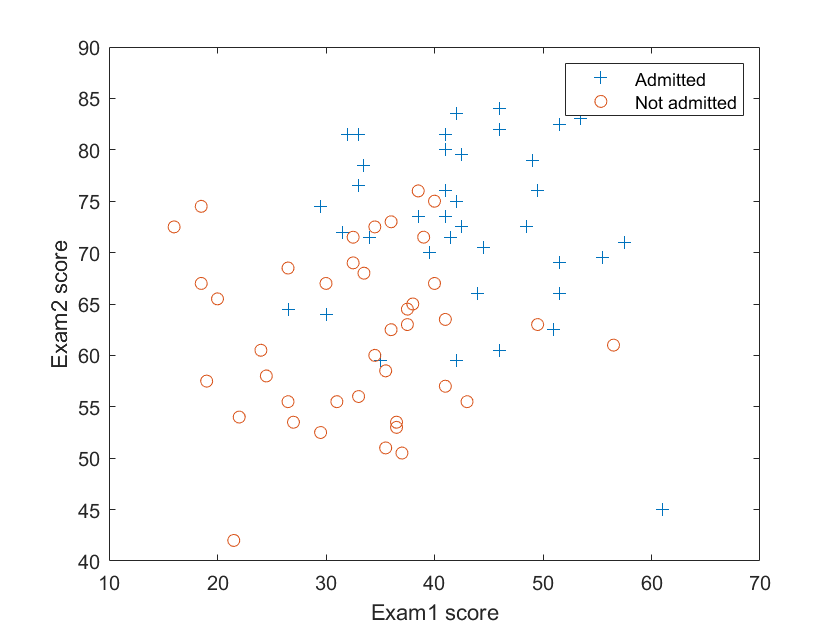
\includegraphics[width=0.7\linewidth]{1.png}
    \caption{数据打印结果}
\end{figure}

\begin{lstlisting}[language=matlab]
    X = load('ex4Data/ex4x.dat');
    Y = load('ex4Data/ex4y.dat');
    
    pos = find(Y == 1);
    neg = find(Y == 0);
    [m, n] = size(X);
    X = [ones(m, 1), X];
    n = n + 1;
    
    plot(X(pos, 2), X(pos, 3), '+');
    hold on;
    plot(X(neg, 2), X(neg, 3), 'o');
    legend('Admitted', 'Not admitted');
\end{lstlisting}

\section{牛顿法迭代收敛Logistic回归}
考虑Logistic二分类问题:
\begin{equation}
    \begin{split}
        P(y=1\;|\;x;\theta)=h_\theta(x)=sigmond(\theta^Tx)=\frac{1}{1+e^{-\theta^Tx}}\in(0, 1)
    \end{split}
\end{equation}

对于数据集$X\in R^{m\times n}, Y\in R^{n}$,设置Cross-Entropy Loss Function为:
\begin{equation}
    \begin{split}
        J(\theta)=\frac{1}{m}\sum_{i=1}^m[-y^{(i)}ln(h_\theta(x^{(i)}))-(1-y^{(i)})ln(1-h_\theta(x^{(i)}))]        
    \end{split}
\end{equation}

然后可以求得Loss Function的梯度为:
\begin{equation}
    \begin{split}
        \nabla J(\theta)=\sum_{i=1}^m[h_\theta(x^{(i)})-y^{(i)}]x^{(i)}=X^T(\hat{Y}-Y)
    \end{split}
\end{equation}

根据牛顿法要求,我们可以最小化Loss Function的二阶泰勒展开式子。即
\begin{equation}
    \begin{split}
        \min_\theta\;J(\theta)\approx \min_\theta\;J(\theta_t)+\nabla J(\theta_t)^T(\theta-\theta_t)+\frac{1}{2}(\theta-\theta_t)^T\nabla^2J(\theta_t)(\theta-\theta_t)\\
    \end{split}
\end{equation}

为使(4)式极小,可以要求其导数为0,即:
\begin{equation}
    \begin{split}
        \frac{dJ(\theta)}{d\theta}=\nabla J(\theta_t)+\nabla^2J(\theta_t)(\theta-\theta_t)=\textbf{0}
    \end{split}
\end{equation}

故有迭代过程:
\begin{equation}
    \begin{split}
        \theta=\theta_t-[\nabla^2J(\theta_t)]^{-1}\nabla J(\theta_t)
    \end{split}
\end{equation}

在Logistic回归中,有
\begin{equation}
    \begin{split}
        \textbf{H}(\theta)=\nabla^2 J(\theta)=\sum_{i=1}^m\frac{\nabla h_\theta(x^{(i)})x^{(i)}}{\nabla \theta}
            =\sum_{i=1}^mx^{(i)}h_\theta(x^{(i)})h_\theta(-x^{(i)})(x^{(i)})^T
    \end{split}
\end{equation}

其中$\textbf{H}$也被称为Hessian Matrix。于是得到迭代过程:
\begin{equation}
    \begin{split}
        \theta = \theta_t - \textbf{H}(\theta_t)^{-1}\nabla J(\theta_t)
    \end{split}
\end{equation}

对应的matlab代码如下:
\begin{lstlisting}[language=matlab]
    X = load('ex4Data/ex4x.dat');
    Y = load('ex4Data/ex4y.dat');

    pos = find(Y == 1);
    neg = find(Y == 0);
    [m, n] = size(X);
    X = [ones(m, 1), X];
    n = n + 1;

    plot(X(pos, 2), X(pos, 3), '+');
    hold on;
    plot(X(neg, 2), X(neg, 3), 'o');

    nIt = 0;
    delta = 1;
    theta = zeros(n, 1);
    while (delta > 1e-6)
        H = X' * diag(sigmond(X * theta) .* sigmond(-X * theta), 0) * X;
        grad = X' * (sigmond(X * theta) - Y);
        theta = theta - H \ grad;
        delta = max(abs(H \ grad));
        nIt = nIt + 1;
    end

    nIt
    xs = 12 : 1 : 63;
    ys = (theta(1) + theta(2) * xs) / (-theta(3));
    plot(xs, ys, 'b-');
    legend('Admitted', 'Not admitted', 'Decision boundary');


    xlabel('Exam1 score');
    ylabel('Exam2 score');
\end{lstlisting}

最终可以得到,仅通过7次迭代就完成了收敛($\theta$变化值小于$10^{-6}$)。得到的$\theta^*=(-16.3787,0.1483, 0.1589)^T$。
(作出$\theta^*)^Tx=0$的图像如下图2所示:
\begin{figure}[h]
    \centering
    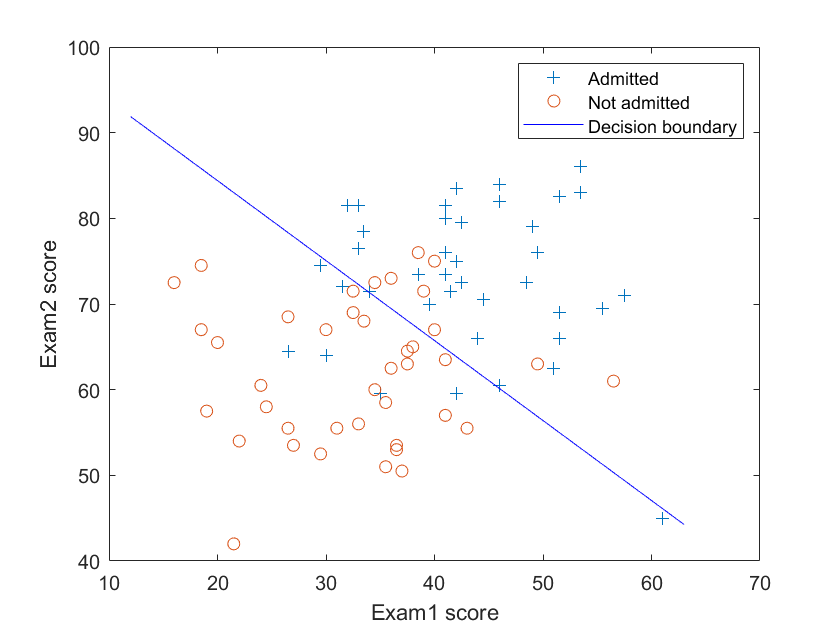
\includegraphics[width=0.7\linewidth]{2.png}    
    \caption{分类结果}
\end{figure}

对于一个Exam 1为20分,Exam 2为80分的同学,预测被录取概率为:
\begin{equation}
    \begin{split}
        P(+1\;|\;(1,20,80)^T;\theta^*)=33.2\%
    \end{split}
\end{equation}

\end{document}